\newpage
\section{Reflexion der Ergebnisse} \label{fazit}
Die in den vorangegangen Kapiteln beschriebenen Analyseansätze und Visualisierungsformen ergeben einen Prototypen für die datengetriebene Analyse und Gestaltung der Berliner Verkehrsinfrastruktur. Durch die gezielte Weiterentwicklung der Analyse sowie der zur interaktiven Datenexploration entwickelten Web-App, könnte ein umfangreiches Werkzeug für Städteplaner und die Berliner Senatsverwaltung für Umwelt, Verkehr und Klimaschutz geschaffen werden. Im Folgenden werden die Projektergebnisse zusammenfassend dargestellt. Ausgehend davon werden die Limitierungen des gewählten Ansatzes beschrieben und mögliche nächste Schritte skizziert.

\subsection{Zusammenfassung der Projektergebnisse}
Die in Kapitel \ref{ergebnisse} gezeigten Analyseansätze ermöglichen eine detaillierte Analyse der in Bezug auf die stark variierende Anbindungsqualität im Stadtgebiet. Ausgehend von der Berechnung der durchschnittlichen Erreichbarkeit fest definierte Bereiche mithilfe von Isochronen, können Unterschiede in der Anbindungsqualität bzw. hinsichtlich der Qualität der vorhandenen Verkehrsinfrastruktur an unterschiedlichen Orten im Stadtgebiet offengelegt werden.

Aus den Ergebnissen ist geht deutlich hervor, dass die innerstädtischen Wohngebiete bereits gut angebunden sind. Bei der Anbindung von Industrie, Gewerbe und Handel gibt es dahingegen Handlungsbedarf. Zudem scheint in den Außenbezirken eine stärkere Verzahnung des bereits bestehenden ÖPNV Angebotes notwendig zu sein. Die Außenbezirke sind häufig auf einzelne Linien sowie einzelne Verkehrsmittel angewiesen.

%Florian L.: Die folgenden auskommentierten Sätze würde ich löschen
% Des Weiteren ist zur besseren Vernetzung unterschiedlicher Verkehrsmittel die Entwicklung und der Ausbau von Mirkomobilitätskonzepten (bspw. Jelbi) zu prüfen und zu fördern.
% Denn nur mit einem breiten diversen Angebot kann die nötige Tiefe und nachhaltige Wende in Berlin eingeleitet werden.​​

% Der Plan zum Ausbau der Straßenbahn in die nord-westlichen Bezirke hat großes Potenzial.
% \todo[inline]{QUELLE FINDEN!!! \% }
% Der Senat hat ähnliche Bedarfe im Süden identifiziert, dieser Bedarf kann ausgehend von der Analyse bestätigt werden.
% \todo[inline]{QUELLE FINDEN!!! \% }

% Wie bereits erwähnt kann damit ein breites Angebot genutzt werden. Dies wiederum führt zu einer Entlastungen in den entsprechenden Verkehrsmitteln oder Angeboten der Mobilität.


% \todo[inline]{MEHR !!! \% mehr Inhalt zur Anreicherung}

\subsection{Limitierungen}\label{limitierung}
\subsubsection{Datenverfügbarkeit und Qualität}
Für die Analyse der Verkehrsinfrastruktur werden, wie in Kapitel \ref{projektumsetzung} beschrieben, hauptsächlich öffentlich zugängliche Geo- und Populationsdaten verwendet. Die genutzten Daten decken jedoch nicht den vollständigen Informationsbedarf für alle detaillierte Analysen, die im Zusammenhang mit innerstädtischer Mobilität durchgeführt werden können. Da diese fehlenden Daten jedoch nicht in ausreichender Qualität und zu mit dem Projektbudget zu vereinbaren Kosten verfügbar waren, leitet sich daraus eine Einschränkung des Analyseumfangs ab. Im Rahmen des Projekts wurden folgende Limitierungen des Analyseumfangs aufgrund mangelnder Datenverfügbarkeit identifiziert:

\begin{itemize}

    \item Die Anzahl der Beschäftigten die in den identifizierten Gewerbe-, Handels- und Industriegebieten tätig sind wird im Zuge der Analyse nicht berücksichtigt. Entsprechende Informationen werden nicht automatisiert erfasst, bzw. stehen nicht öffentlich zur Verfügung. Durch die Berücksichtigung von Beschäftigtenzahlen könnten Aussagen über das zu erwartende Auslastung der Verkehrsinfrastruktur in bestimmten Teilen des Stadtgebiets getroffen werden.

    \item Die Betrachtung der Auslastung des ÖPNV ist nicht Teil des aktuellen Projekts. Entsprechende Daten sind nicht öffentlich zugänglich. Die Betrachtung der aktuellen Auslastung ist für die Dimensionierung neuer ÖPNV-Vorhaben unerlässlich.

    \item Die Taktung des ÖPNV wird in der Analyse nicht berücksichtigt​. Eine zuverlässige und effiziente Einbindung entsprechender Daten waren aufgrund der limitierten Ressourcen im Rahmen des Projekts nicht möglich.

    \item Die Daten zu den tatsächlichen Geschwindigkeiten des Autoverkehrs liegen nicht für alle Straßenabschnitte/-segmente vor​. Durch die weitere Anreicherung der im Projekt genutzten Daten um weitere Straßensegmente, könnte eine die Analyse des Straßenverkehrs weiter detailliert werden.

    \item Die Barrierefreiheit von Haltestellen wird aufgrund fehlender Daten nicht berücksichtigt​. Die Verfügbarkeit entsprechender Daten ist die Voraussetzung dafür, dass bei der Berechnung der Anbindungsqualität auch die Bedürfnisse von Bürger*innen mit eingeschränkter Mobilität berücksichtigt werden können.

    \item Es werden weder Hausbote, noch gewerbliche Flächen und Verkehrsmittel auf Wasserflächen in der Analyse berücksichtigt. Insbesondere die durch die BVG betriebenen Fähren könnten im weiteren Verlauf in die Analyse mit aufgenommen werden, um den Detailgrad weiter zu steigern.

\end{itemize}

\todo[inline]{Wenn was fehlt: Bitte ergänzen}

\subsubsection{Komplexität der Analyse}
Ausgehend von der limitierten Datenverfügbarkeit und -qualität sowie den limitierten Ressourcen ergeben sich auch hinsichtlich der Komplexität der Analyse Limitierungen.

\begin{itemize}

    \item Die Bestimmung der Anbindungsqualität wird im Rahmen des Projekts ausschließlich durch die Berechnung der Erreichbarkeit auf Basis von Isochronen vorgenommen. Durch die Anreicherung um die Taktung des ÖPNV sowie die Auslastung der vorhandenen Verkehrsinfrastruktur, würde die Anbindungsqualität weiter an Aussagekraft gewinnen.

    \item Bei der Berechnung der Anbindungsqualität werden keine „Penalty“ eingerechnet. So werden weder für die Nutzung des Autos Zeiten für die Parkplatzsuche, noch bei der Nutzung des ÖPNV Zeiten für Umstiege (bspw. für die Wegstrecke von einer U-Bahnlinie zu einer S-Bahnlinie)berücksichtigt.
    \item Aktuell werden ausschließlich 15 Minuten Isochrone analysiert​. Die Berechnung von Isochronen ist ressourcenintensiv, sodass zwischen der Berechnung unterschiedlicher Isochrone abgewogen werden musste. Die 15 Minuten Isochrone eignen sich besonders zur Berechnung der Anindungsqualität, weil ...
\end{itemize}
\todo[inline]{Wenn was fehlt: Bitte ergänzen; letzten Bulletpoint vervollständigen}


\subsubsection{Begrenztes Domänenwissen}
Im Rahmen des Projekts wurden Expert*innen der Senatsverwaltung für Umwelt, Verkehr und Klimaschutz punktuell in die Entwicklung des Prototyps eingebunden. Für die Weiterenwicklung des Analyseansatzes ist eine stärkere Einbeziehung von Domänenwissen notwendig. Entsprechendes Domänenwissen wird auch auch für die Validierung der in Kapitel \ref{ergebnisse} vorgestellten Handlungsvorschläge vorausgesetzt.

\todo[inline]{Wenn was fehlt: Bitte ergänzen}

\subsection{Ausblick}

\subsubsection{Anreicherung der Analyse}
Die Anreicherung der Analyse - ausgehend von den in den Kapiteln 5.2.1 und 5.2.2 beschriebenen Limitierungen - würde die  Genauigkeit der Prädiktionen der Analyse weiter steigern. Demnach sollte eine Erweiterung der Datengrundlage sowie eine Steigerung der Analysekomplexität angestrebt werden. Insbesondere die Berücksichtigung von Datenpunkten bezüglicher der Taktung und Auslastung des ÖPNV wäre zielführend. Zudem würde die Einbindung von „Penaltys“ (bspw. Zeit für die Parkplatzsuche bei Nutzung eines PKW) eine Feinjustierung des Analyseansatzes ermöglichen.

\todo[inline]{Wenn was fehlt: Bitte ergänzen, Referenz zu den Kapiteln 5.2.1 und 5.2.2 richtig formatieren}

\subsubsection{Finalisierung des interaktiven Mobililitätskompasses}
Wie in Kapitel \ref{website} beschrieben, verfügt der Prototyp bereits heute über einen interaktiven Modus. Mithilfe des interaktiven Mobilitätskompasses, bzw. Dashboards lassen sich individuelle Analysen der Verkehrsinfrastruktur durchführen. In Kapitel \ref{einleitung} wird dargelegt, dass die fehlende Einbindung der Bürger*innen zu Kritik an der Umsetzung des Mobilitätsgesetzes führt. Durch den gezielten Ausbau des interaktiven Mobilitätskompasses könnte ein Werkzeug für die die Bürger*innenkommunikation geschaffen werden, welches von Bürger*innen genutzt werden könnte um sich über den aktuellen Stand der Verkehrsinfrastrukutr zu erkundigen. Auf diese Weise könnten Bürger*innen die Notwendigkeit einzelner Infrastrukturmaßnahmen gezielt nachvollziehen. Es könnte auch ein Votingsystem zur Priorisierung von Infrastrukturmaßnahmen eingeführt werden, um das Gefühl der Teilhabe zu steigern.

\todo[inline]{Wenn was fehlt: Bitte ergänzen; Abbildung unten richtig formatieren}

\img{dashboard001}{dashboard001}{width=14cm}{individuelles Dashboard (eigene Darstellung)}

\subsubsection{Entwicklung eines Planungstools}
Der interaktive Mobilitätskompass dient zudem als Ausgangspunkt für die Entwicklung eines umfangreichen Planungstools für Städteplaner und Entscheider*innen in der Berliner Senatsverwaltung für Umwelt, Verkehr und Klimaschutz. Zusätzlich zu der deskriptiven Analyse der Ist-Situation könnten beispielsweise Streckenverläufe die sich noch in der Planung befinden, in die Graphen-Struktur eingepflegt werden. Auf diese Weise könnte simuliert werden, wie sich die Realisierung eines bestimmten Infrastrukturprojekts (bspw. die Erweiterung einer S-Bahnstrecke) auf die Anbindungsqualität im betroffenen Stadtgebiet auswirken würde. Dadurch könnten die Potenziale von Infrastrukturvorhaben unkompliziert und visuell evaluiert werden.

\todo[inline]{Wenn was fehlt: Bitte ergänzen}

\subsubsection{Entwicklung eines Mobilitätsindexes}\label{mobwob_index}
Durch die fortlaufende Erweiterung und Aktualisierung der Datengrundlage könnte auf Basis des, in den Kapiteln \ref{projektumsetzung} und \ref{ergebnisse} vorgestellten, Analyseansatz ein fortlaufender Mobilitätsindex entwickelt werden. Unter Berücksichtigung relevanter Faktoren wie Handels-, Industrie- und Gewerbedichte, Einwohnerdichte, Taktung, Verfügbarkeit und Geschwindigkeit könnten der Mobilitätsindex eingesetzt werden um Veränderungen in der Anbindungsqualität über die Zeit feststellen zu können und um weitere Maßnahmen zu identifizieren. 

Die Entwicklung eines Mobilitätsindexes mit Fokus auf die durch die Verkehrsinfrastruktur gewährleistete Anbindungsqualität, wäre eine wertvolle Ergänzung zum bestehenden Bundesländerindex Mobilität \& Umwelt.\footcite{Bundeslaenderindex:1}

Der Bundesländerindex Mobilität \& Umwelt bewertet die Verkehrsinfrastruktur auf Ebene der Bundesländer entlang der Faktoren Verkehrssicherheit, Lärmminderung, Flächenverbrauch, Klimaschutz und Luftqualität (siehe Abbildung~\ref{mob-index2018}).

\img{mob-index2018}{mob-index2018}{width=14cm}{Bundesländerindex Mobilität \& Umwelt Ergebnisse \footcite{Bundeslaenderindex:4}}

Analog zum Bundesländerindex Mobilität \& Umwelt könnte der Mobilitätsindex durch eine entsprechende Anreicherung der Datengrundlage dahingehend ausgestaltet werden, dass der laufende Vergleich (Monitoring) der Anbindungsqualität auf Ebene der Bundesländer oder Städte möglich ist.

\img{mob-index2018-Verteilung}{mob-index2018-Verteilung}{width=14cm}{Bundesländerindex Mobilität \& Umwelt Gewichtung \footcite{Bundeslaenderindex:4}}

Die gezeigte Verteilung verdeutlicht wie der Bundesmobilitätsindex gewichtet wurde. Es wird dazu konstruktiv der folgende Vorschlag unterbreitet, der nur ein Minimum an Ergänzungen darstellt.

\img{mob-index-anpassung}{mob-index-anpassung}{width=14cm}{Mobilitätsindex ergänzt und erweitert (eigene Darstellung)}

Die Erweiterung, in Abbildung~\ref{mob-index-anpassung} dargestellt, sieht unteranderem eine andere Gewichtung vor. Vor allem sollten die genutzten Flächen einen höheren Beitrag zur Bewertung aufweisen. Dies kann die Korrelation zwischen dicht besiedelten Gebieten und der Luftqualität ggf. abschwächen aber auch die CO2 Emittierung von dichten Industrieansiedlungen in dem Bundesland oder dem Stadtstaat.
Am wichtigsten ist aber mitunter das einführen einer neuen Datenquelle bzw. einer neuen Dimension. Der öffentliche Nahverkehr und der regionale Überlandverkehr ist besonders in nicht dicht besiedelten Gebieten essentiell.
Das abbilden des Ausbaus der Nutzung etc. zeigt in einem stetigen Mobilitätsindexes auch deren Entwicklung an und kann als Werkzeug zur Transparenz genutzt werden.
Des Weiteren lassen sich mit einer immer komplexeren Formalisierung eines ganzheitlichen Indexes Städte, Bundesländer oder sogar Landkreise vergleichen. Das ermöglicht Planern aber auch Förderer, Mittel und Maßnahmen an der bzw. den geeigneten Stellen zu platzieren.


\todo[inline]{Quelle für den Mob. Index (footcite und Bild) zu einer neueren Quelle aktualisieren, Abbildungsverweis einbauen, ggf. Abbildung zur Hervorhebung möglicher Faktoren die bei unseren Mobilitätsindex einfließen könnten erstellen .... CHECK, CHECK und CHECK .. letzteres sieht aber noch nicht Hipp genug aus!!! ... pptx mit dem Text liegt im abbildungs Ordner}

% Kommentar von Florian L.: Den folgenden Text würde ich rausnehmen. Habe den Teil überarbeitet und im Absatz oberhalb aufgeriffen.

% Mit mehr Ressourcen könnte auch die Ausweitung oder Reduzierung der Domäne betrachtet werden. Darunter zählt die Urbanisierung sowie die Suburbanisierung.
% Ersteres ist die allgemeinbekannte Landflucht und letzteres ist die Stadflucht. Beide beschreiben die Veränderung von Regionen oder Domänen.
% Diese Einflussnahme sollte mit Experten zusammen weiter betrachtet werden und ggf. Maßnahmen für eine Stabilisierung bzw. für ein sinnvolles Gleichgewicht in der Urbanisierung oder Suburbanisierung gefunden werden.

% Auch die Sozioökonomischen und ökologischen Perpektiven sollten vertieft werden.
% %Letzteres kann den Forstämtern dabei helfen Wild und deren Pupolation besser zu Steuern aber auch das schaffen neuer Räume für gefärdete Arten zeitig auszuschreiben.
% Den nicht trennscharf eingeführten Begriff der Sozioökonomie könnte unteranderem die Entwicklung eines fortlaufenden Mobilitätsindex, um Veränderungen in der Anbindungsqualität feststellen zu können und zur Identifizierung weitere weitere Maßnahmen.

% \todo[inline]{AUFFÜHREN UND QUELLEN NUTZEN !!! \% aufzeigen das keine Trennschärfe existiert und ggf. ein oder zwei Aussagen hinzufügen}

% Hierbei könnten sowohl Ökologische aber auch Ökonomische Aspekte verstärkt gewichtet werden. %Damit könnten sich die Bewohner oder Nutzer einer Domäne vielleicht besser identifizieren.
% Auch der Vergleich mit anderen Städten oder Landkreisen könnte hier wichtig sein. Es wurde nur der Ballungsraum Berlin betrachtet und das Umland wurde nicht betrachtet. Das schmälert das Gewicht der Pendler. Alles in Allem muss der Mobilitätsindex Formalisiert werden.

% Gewichte die in einem Mobilitätsindex ein Rolle spielen könnten unter anderm Anteil an Miet- und Eigentumswohnungen sowie die Einwohner-,
% Gewerbe oder Industriedichte. Auch die durchschnittliche Geschwindigkeit aller möglichen Verkehrsmittel,
% die ÖPNV Streckendichte (verschiedene Medien summieren), die ÖPNV Haltestellendichte oder die Straßendichte mit Fahrradwegen und PKW/LKW Wegen.
% Als negativbeispiel kann der formalisierte Mobilitätsindex genannt werden.

%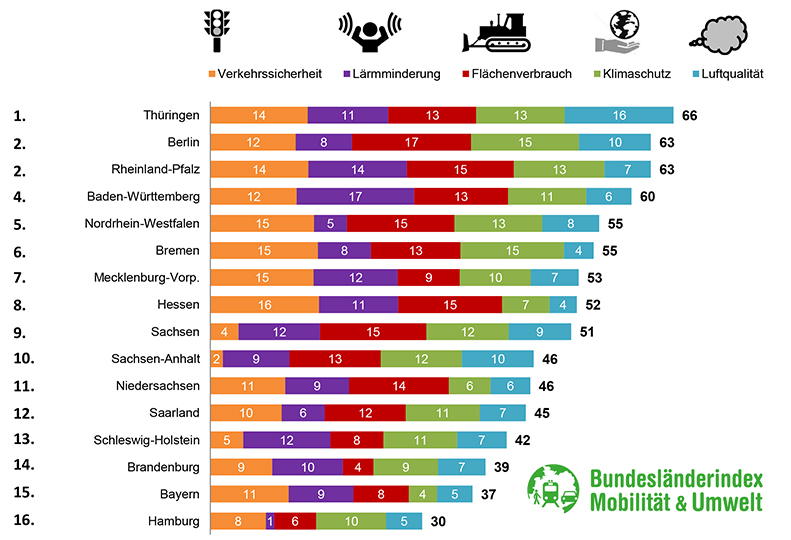
\includegraphics{​​​​../abbildungen/Mob-Index.jpg}
%\includegraphics[width=11cm]{abbildungen/mob-index} \\
%\img{mob-index}{width=14cm}{Mobilitätsindex \footcite{Bundeslaenderindex:3}}
%\img{​​​​mob-index}​{​​​​width=11cm}​​​​{​​​​Mobilitätsindex}​​​​

%\cite{DUMMY:1}
%\footcite{Bundesländerindex:3}
